\subsection{Problem 2: Dua Nakhoda, Satu Kapal}

\subsubsection{Identifikasi Masalah}

Pada Milestone 1, Aggregator berjalan sebagai instans tunggal yang memegang kendali penuh atas jadwal \textit{polling} ke BMKG dan PVMBG. Pada Milestone 2, sistem diskalakan menjadi minimal tiga instans agar sanggup melayani beban baca tinggi dan bertahan dari kegagalan mesin. Perubahan ini melahirkan empat persoalan utama sistem terdistribusi:

\begin{enumerate}
  \item \textbf{Duplikasi pengambilan data akibat banyak instans tanpa pemimpin tunggal (Kriteria 1 dan 2).}
  Jika tiga replika Aggregator langsung berjalan tanpa koordinasi, ketiganya akan menghubungi BMKG dan PVMBG secara bersamaan. Sumber hulu akan menerima permintaan berlipat ganda dan penulisan data serentak rawan memicu \textit{race condition} serta duplikasi. Dalam literatur sistem terdistribusi, persoalan ini diselesaikan memakai pola \textbf{\textit{leader election}}, \textbf{\textit{single-active poller}}, dan \textbf{\textit{distributed lease}}.

  \item \textbf{Kegagalan koordinasi akibat pergeseran jam \textit{node} (Kriteria 4).}
  Jadwal atau sewa berbasis jam lokal (\textit{wall-clock}) mengasumsikan jam seluruh mesin selalu sinkron melalui NTP. Jika sinkronisasi waktu suatu \textit{node} berhenti dan jamnya bergeser maju atau mundur, pemegang sewa bisa salah menilai masa kedaluwarsa. Node yang jamnya melambat akan mengira sewanya belum habis, sementara \textit{node} yang jamnya melompat maju dapat salah mengambil alih peran. Persoalan ini dikenal sebagai \textbf{\textit{clock skew}}, yang menuntut penggunaan sumber waktu tunggal yang otoritatif dan \textit{monotonic clock}.

  \item \textbf{Fenomena \textit{zombie leader} setelah jeda proses atau pembekuan VM (Kriteria 5).}
  Walaupun jam seluruh \textit{node} sudah sinkron, suatu proses atau VM dapat membeku lebih lama daripada masa berlaku \textit{lease}. Saat \textit{node} itu aktif kembali, ia dapat mengira dirinya masih pemimpin dan mengirim operasi tulis usang padahal pemimpin baru sudah bekerja. Dalam literatur, kondisi ini disebut \textbf{\textit{split-brain}} atau \textbf{\textit{stale zombie writer}}. Solusinya memadukan pembatalan lokal berpatokan jam monotonik dengan \textbf{\textit{monotonic fencing tokens}} yang diverifikasi atomik oleh basis data.

  \item \textbf{Penskalaan dinamis dan pembaruan versi tanpa permintaan gagal (Kriteria 6, 7, dan 8).}
  Jumlah replika Aggregator akan diubah saat pengujian beban berlangsung dan versi layanannya diperbarui secara bertahap. Mematikan \textit{pod} secara mendadak sebelum mengeluarkannya dari daftar tujuan \textit{load balancer} akan memutus koneksi aktif dan menaikkan \textit{error rate}. Persoalan ini menuntut \textbf{\textit{graceful shutdown}} atau \textit{connection draining} serta strategi \textbf{\textit{zero-downtime rolling update}}.
\end{enumerate}

\subsubsection{Rancangan Solusi dan Mekanisme yang Dipilih}

Rancangan Problem 2 memisahkan peran \textbf{layanan baca} dari peran \textbf{\textit{poller} aktif}. Seluruh replika Aggregator tetap aktif melayani permintaan baca dari Client API agar kapasitas pemrosesan meningkat, tetapi hanya satu replika pemegang \textit{lease} yang mengambil data dari tiap sumber hulu. Arsitektur ini diperlihatkan pada \textbf{Gambar~\ref{fig:p2-arch}}.

\begin{figure}[H]
  \centering
  \IfFileExists{figures/p2-arsitektur-koordinasi.png}{%
    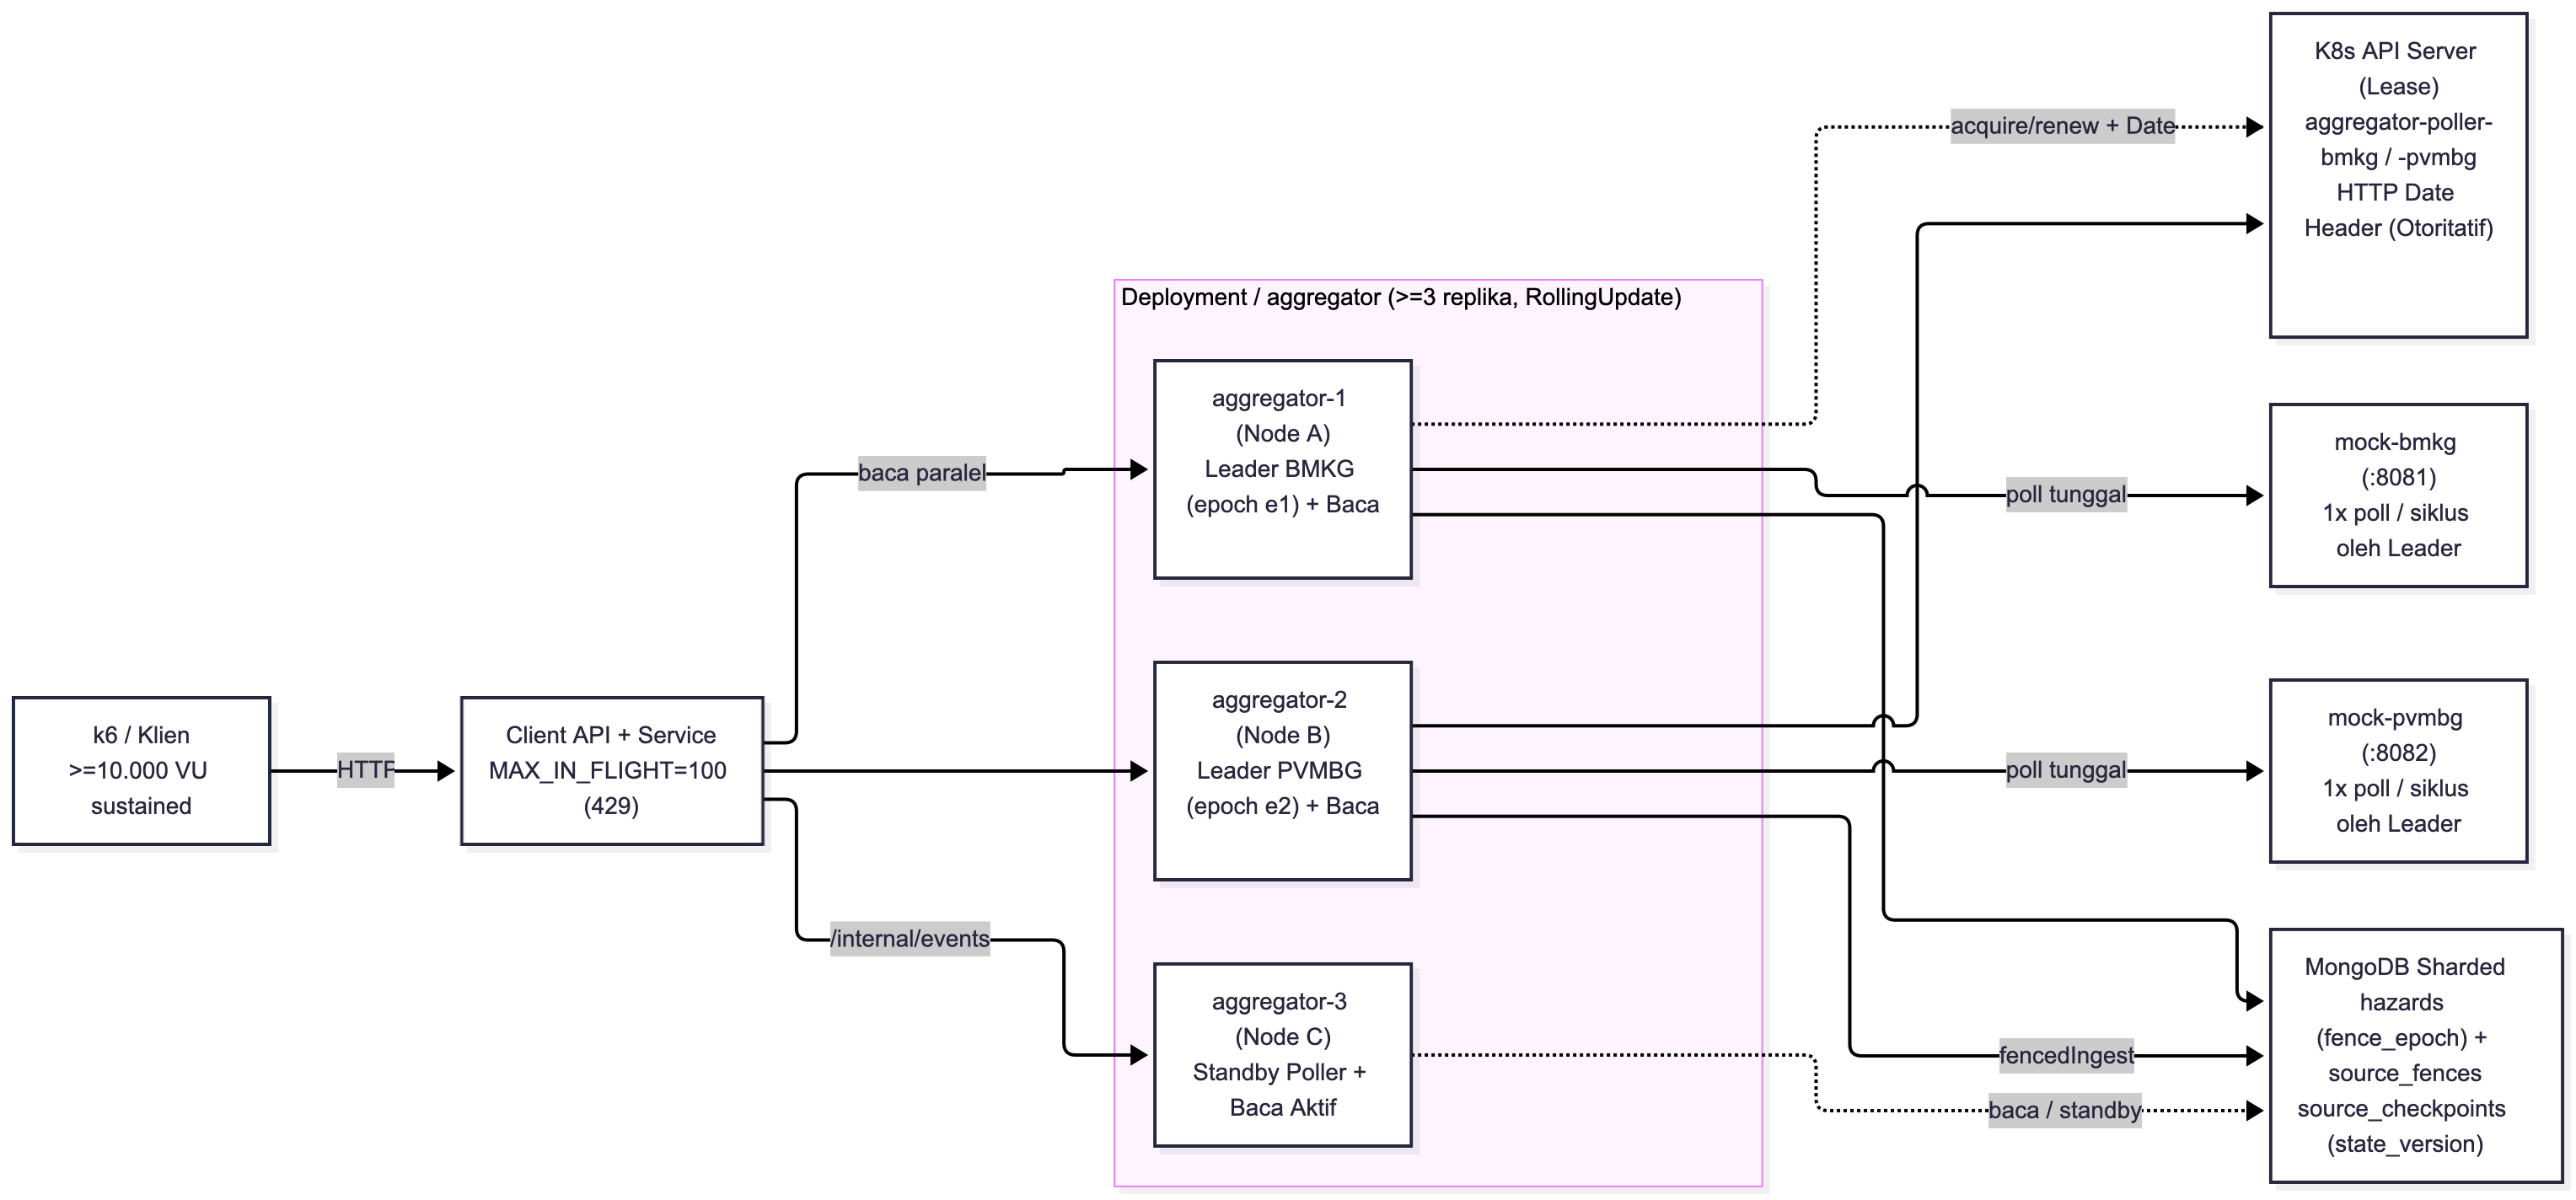
\includegraphics[width=0.95\linewidth]{p2-arsitektur-koordinasi.png}%
  }{%
  \resizebox{\linewidth}{!}{%
  \begin{tikzpicture}[
    every node/.style={font=\sffamily\footnotesize},
    box/.style={draw=black!65, rounded corners=3pt, fill=white, align=center, inner sep=5pt, minimum width=3.1cm, minimum height=0.88cm},
    leader/.style={draw=green!50!black, rounded corners=3pt, fill=green!7, align=center, inner sep=5pt, minimum width=3.1cm, minimum height=0.88cm},
    store/.style={draw=blue!55!black, rounded corners=2pt, fill=blue!6, align=center, inner sep=5pt, minimum width=3.2cm, minimum height=0.88cm},
    group/.style={draw=black!35, dashed, rounded corners=4pt, fill=black!2, inner sep=9pt},
    arr/.style={-{Stealth[length=2.2mm]}, thick, draw=black!75},
    lbl/.style={font=\sffamily\scriptsize, fill=white, inner sep=1.5pt, align=center}
  ]
    % Kiri: Klien & Load Balancing
    \node[box] (k6)  at (0, 2.2) {\textbf{k6 / Klien}\\{\scriptsize $\ge$10.000 VU sustained}};
    \node[box] (capi) at (4.4, 2.2) {\textbf{Client API + Service}\\{\scriptsize MAX\_IN\_FLIGHT=100 (429)}};

    % Tengah: 3 Replika Aggregator
    \node[leader] (agg1) at (10.2, 4.4) {\textbf{aggregator-1 (Node A)}\\{\scriptsize Leader BMKG (epoch $e_1$) + Baca}};
    \node[leader] (agg2) at (10.2, 2.2) {\textbf{aggregator-2 (Node B)}\\{\scriptsize Leader PVMBG (epoch $e_2$) + Baca}};
    \node[box]    (agg3) at (10.2, 0.0) {\textbf{aggregator-3 (Node C)}\\{\scriptsize Standby Poller + Baca Aktif}};

    % Atas: Kubernetes Lease Authority
    \node[store] (k8s) at (17.6, 5.8) {\textbf{K8s API Server (Lease)}\\{\scriptsize aggregator-poller-bmkg / -pvmbg}\\{\scriptsize HTTP Date Header (Otoritatif)}};

    % Kanan Tengah: Sumber Upstream
    \node[box] (bmkg)  at (17.6, 3.6) {\textbf{mock-bmkg (:8081)}\\{\scriptsize 1x poll / siklus oleh Leader}};
    \node[box] (pvmbg) at (17.6, 1.9) {\textbf{mock-pvmbg (:8082)}\\{\scriptsize 1x poll / siklus oleh Leader}};

    % Kanan Bawah: MongoDB Fencing & Checkpoint
    \node[store] (db) at (17.6, -0.2) {\textbf{MongoDB Sharded}\\{\scriptsize hazards (fence\_epoch) + source\_fences}\\{\scriptsize source\_checkpoints (state\_version)}};

    % Grouping
    \begin{scope}[on background layer]
      \node[group, fit=(agg1)(agg2)(agg3), label={[font=\sffamily\scriptsize\bfseries]below:Deployment/aggregator ($\ge$3 replika, RollingUpdate)}] (aggrp) {};
    \end{scope}

    % Panah baca (ke semua replika)
    \draw[arr] (k6) -- node[lbl, above] {HTTP} (capi);
    \draw[arr] (capi.east) -- ++(0.9,0) |- node[lbl, near end, above] {baca paralel} (agg1.west);
    \draw[arr] (capi.east) -- (agg2.west);
    \draw[arr] (capi.east) -- ++(0.9,0) |- node[lbl, near end, below] {/internal/events} (agg3.west);

    % Panah lease (semua replika bersaing/renew)
    \draw[arr, dashed] (agg1.north) |- node[lbl, pos=0.72, above] {acquire/renew + Date} (k8s.west);
    \draw[arr, dashed] ([yshift=2mm]agg2.east) -- ++(1.1,0) |- ([yshift=-2mm]k8s.west);

    % Panah poll tunggal (hanya leader)
    \draw[arr] (agg1.east) -- ++(1.3,0) |- node[lbl, pos=0.72, above] {poll tunggal} (bmkg.west);
    \draw[arr] (agg2.east) -- node[lbl, above] {poll tunggal} (pvmbg.west);

    % Panah fenced write & checkpoint
    \draw[arr] ([yshift=-2mm]agg1.east) -- ++(0.7,0) |- ([yshift=3mm]db.west);
    \draw[arr] ([yshift=-2mm]agg2.east) -- ++(0.45,0) |- node[lbl, pos=0.25, right] {fencedIngest} (db.west);
    \draw[arr, dashed] (agg3.east) -- ++(1.4,0) |- node[lbl, pos=0.72, below] {baca / standby} ([yshift=-3mm]db.west);
  \end{tikzpicture}%
  }%
  }
  \caption{Diagram Rancangan Koordinasi Leader, Fencing, dan Penskalaan Problem 2}
  \label{fig:p2-arch}
\end{figure}

Rancangan ini diwujudkan melalui empat mekanisme utama berikut.

\paragraph*{1. Pemilihan Pemimpin per Sumber Berbasis Kubernetes \texttt{Lease}}
Koordinasi kepemilikan dikelola oleh \texttt{SourceLeaderManager} (\path{aggregator/src/coordination/leaderLoop.ts}). Pada \path{aggregator/src/index.ts:979-1010}, sistem menjalankan dua instans terpisah untuk \texttt{aggregator-\allowbreak poller-\allowbreak bmkg} dan \texttt{aggregator-\allowbreak poller-\allowbreak pvmbg}. Pemisahan ini mendistribusikan beban \textit{polling} BMKG dan PVMBG ke dua replika berbeda secara alami.

\begin{itemize}
  \item \textbf{Sumber waktu otoritatif (\path{aggregator/src/coordination/lease.ts:53-287}):} pada mode \path{COORDINATION_MODE=k8s}, kelas \texttt{Kubernetes\allowbreak Lease\allowbreak Provider} memakai objek \path{coordination.k8s.io/v1} \texttt{Lease}. Penilaian masa kedaluwarsa mengacu pada \textit{header} HTTP \texttt{Date} milik Kubernetes API Server (\texttt{serverNowMs}). Pada mode \path{COORDINATION_MODE=db}, \texttt{MongoLeaseProvider} memakai \texttt{hello.localTime} dari MongoDB. Dengan rancangan ini, jam sistem lokal \textit{node} tidak pernah menentukan masa berlaku \textit{lease}.
  \item \textbf{Penjaga pembaruan monotonik lokal (\path{leaderLoop.ts:75-104}):} setiap \textit{pod} memantau keterlambatan pembaruannya memakai jam monotonik proses (\texttt{performance.now()}). Bila \textit{node} mengalami pembekuan VM sehingga selisih pembaruan beserta batas aman ($2.500\text{ ms}$ untuk BMKG dan $5.500\text{ ms}$ untuk PVMBG) melewati \texttt{renewDeadlineMs} (\texttt{12 detik}), \texttt{Source\allowbreak Leader\allowbreak Manager} langsung mencabut status pemimpin lokal dan membatalkan siklus lewat \texttt{AbortSignal}.
\end{itemize}

\paragraph*{2. \textit{Monotonic Epoch Fencing} dan \textit{Checkpoint} Optimistik}
Pembatalan lokal saja belum menutup risiko jeda sesaat sebelum panggilan jaringan terkirim. Oleh karena itu, seluruh penulisan ke basis data dilindungi pagar generasi monotonik (\path{aggregator/src/coordination/fencing.ts}) serta \textit{checkpoint} berversi (\path{aggregator/src/coordination/checkpoints.ts}).

\begin{enumerate}
  \item \textbf{Penaikan \textit{epoch} saat transisi (\texttt{activateEpoch}, baris 31--44):} tiap kali memperoleh kepemilikan \textit{lease} baru, Aggregator menaikkan nilai \texttt{epoch} secara atomik lewat \texttt{\$inc: \{ epoch: 1 \}} pada koleksi \path{source_fences}.
  \item \textbf{Penulisan berpagar dua lapis (\texttt{fencedIngest}, baris 86--112):} sebelum menulis, fungsi memeriksa validitas lokal dan memverifikasi \texttt{fenceStore.assertEpoch(source, epoch)}. Di sisi dokumen kanonik (\path{mongoRepository.ts:88, 95}), syarat atomik \path{fence_epoch: { $lte: epoch }} langsung menolak \textit{zombie leader} ber-\textit{epoch} lama dengan status \texttt{stale\_epoch}. Jika \textit{epoch} berganti tepat sesudah dokumen terbuat, pemeriksaan ulang menghapus dokumen yatim itu lewat \texttt{repo.remove}.
  \item \textbf{\textit{Checkpoint} tanpa celah (\texttt{MongoCheckpointStore.commit}, baris 29--68):} kursor tersimpan di \path{source_checkpoints} dengan syarat \texttt{state\_version} dan \texttt{owner\_epoch: \{ \$lte: next.owner\_epoch \}}. Pemimpin baru otomatis menyambung dari \texttt{committed\_offset}, sementara pemimpin lama gagal memperbarui kursor.
\end{enumerate}

\begin{lstlisting}
// aggregator/src/coordination/fencing.ts:95-111
const source = input.event.source;
const stillValidBefore = await fenceStore.assertEpoch(source, input.epoch);
if (!stillValidBefore) {
    return { outcome: 'stale_epoch', hazard_id: input.event.hazard_id, detail: 'superseded by newer epoch' };
}

const res = await repo.ingest(input);
if (res.outcome !== 'applied') return res;

const stillValidAfter = isLocalLeaderStillValid() && (await fenceStore.assertEpoch(source, input.epoch));
if (!stillValidAfter) {
    if (res.created) {
        await repo.remove(res.hazard_id, input.epoch).catch(() => undefined);
    }
    return { outcome: 'stale_epoch', hazard_id: res.hazard_id, detail: 'epoch changed during write' };
}
return res;
\end{lstlisting}

\paragraph*{3. Penskalaan Horizontal, Pengurasan Koneksi, dan Pembaruan Bertahap}
Untuk mendukung penskalaan $3 \to 5 \to 2$ serta pergantian versi tanpa permintaan gagal, sistem menerapkan tiga pengaturan pada manifest dan layanan.

\begin{itemize}
  \item \textbf{Sebaran \textit{pod} Kubernetes (\path{k8s/base/aggregator/workload.yaml}):} jumlah awal disetel tiga replika memakai \texttt{topologySpreadConstraints} beropsi \texttt{ScheduleAnyway} agar skala lima replika pada tiga VM tetap berjalan. Akses ke objek \texttt{leases} diatur lewat \texttt{Role} bernama \path{aggregator-lease-role}.
  \item \textbf{\textit{RollingUpdate} dan \textit{graceful drain}:} \textit{deployment} memakai \texttt{maxSurge: 1} dan \texttt{maxUnavailable: 0} supaya kapasitas tidak pernah turun saat pembaruan versi. Kait \texttt{preStop: sleep 5} memberi waktu bagi Kubernetes untuk melepas IP \textit{pod} dari layanan. Sementara itu, penangan \texttt{SIGTERM} mengubah \path{/health} menjadi \texttt{503}, melepas \textit{lease} lewat \texttt{stop()}, dan menuntaskan koneksi lewat \texttt{server.close}.
  \item \textbf{Pembatas beban pada \texttt{client-api} (\path{client-api/src/index.ts:20}):} \textit{middleware} \texttt{inFlightLimit} (\path{MAX_IN_FLIGHT=100}) membalas kelebihan beban secara terkontrol dengan **HTTP 429** agar \textit{pod} tidak kehabisan memori.
\end{itemize}

\paragraph*{4. Parameter \textit{Lease} dan Konfigurasi \textit{Load Testing}}
Parameter bawaan waktu sewa ditetapkan pada \path{k8s/base/aggregator/kustomization.yaml:13-16} dan \path{.env.example:85-88}. Nilai \path{LEASE_DURATION_SEC} bernilai \texttt{20} detik, \path{LEASE_RENEW_DEADLINE_SEC} bernilai \texttt{12} detik, dan \path{LEASE_RETRY_PERIOD_SEC} bernilai \texttt{3} detik.

Dengan komposisi ini, waktu maksimum pengambilalihan oleh pemimpin baru saat pemimpin lama mati mendadak adalah sekitar $20 + 3 = 23\text{ detik}$, jauh di bawah batas $60\text{ detik}$. Dalam kondisi normal, pemimpin berkesempatan memperbarui \textit{lease} hingga empat kali di dalam rentang $12\text{ detik}$ dengan selisih aman $8\text{ detik}$.

Pengujian beban memakai \texttt{k6} pada \path{load-test/p2-scale.js} dari luar \textit{pod} aplikasi. Skrip membangkitkan \texttt{10.000} \textit{virtual user} selama \texttt{120 detik}, menyegarkan token setiap 45 detik sebelum masa aktif 60 detik habis, dan mengizinkan kode status \texttt{200} serta \texttt{429} dengan ambang \path{http_req_failed: ['rate<0.01']}.

\subsubsection{Alasan Keputusan}

\textbf{Tabel~\ref{tab:p2-decisions}} merangkum keputusan desain Problem 2, alasan dan konsekuensinya, serta alternatif yang ditolak.

\begin{small}
\begin{longtable}{@{} >{\raggedright\arraybackslash}p{3.4cm} >{\raggedright\arraybackslash}p{7.4cm} >{\raggedright\arraybackslash}p{4.0cm} @{}}
  \caption{Desain, Alasan, dan Alternatif yang Ditolak pada Problem 2}
  \label{tab:p2-decisions} \\
  \toprule
  \textbf{Keputusan} & \textbf{Alasan} & \textbf{Alternatif (Ditolak)} \\
  \midrule
  \endfirsthead
  \caption[]{Desain, Alasan, dan Alternatif yang Ditolak pada Problem 2 (Lanjutan)} \\
  \toprule
  \textbf{Keputusan} & \textbf{Alasan} & \textbf{Alternatif (Ditolak)} \\
  \midrule
  \endhead
  \midrule
  \multicolumn{3}{r}{\textit{Bersambung ke halaman berikutnya...}} \\
  \endfoot
  \bottomrule
  \endlastfoot
  \textit{Lease} berbasis HTTP \texttt{Date} otoritatif plus jam monotonik \texttt{performance.\-now()} & Menggunakan satu sumber waktu otoritatif mencegah kesalahan akibat \textit{clock skew} antar-\textit{node}. Penggunaan \texttt{performance.now()} memastikan jeda proses atau pembekuan VM langsung membatalkan kepemimpinan lokal. Konsekuensinya, Aggregator memerlukan izin RBAC \texttt{coordination.k8s.io/leases}. & \textbf{Membandingkan jam dinding lokal antarpod:} langsung gagal saat sinkronisasi waktu satu \textit{node} terhenti. \textbf{Menjalankan klaster Raft internal di Node.js:} menambah kerumitan konsensus baru di luar Kubernetes. \\
  \midrule
  Menambahkan \textit{epoch fencing} (\path{source_fences}) dan \textit{checkpoint} versi (\path{source_checkpoints}) & \textit{Lease} saja belum cukup karena proses yang baru bangun tetap dapat mengirim operasi tulis usang ke jaringan. Validasi \texttt{fence\_epoch} dan \texttt{owner\_epoch} secara atomik menutup celah \textit{zombie writer} dengan biaya tambahan satu kali cek \textit{epoch}. & \textbf{Hanya mengandalkan pembatalan \textit{lease} di sisi klien:} masih menyisakan peluang \textit{race condition} antara saat \textit{lease} berpindah dan saat penulisan tiba di basis data. \\
  \midrule
  Memisahkan objek \texttt{Lease} per sumber (\texttt{-bmkg} dan \texttt{-pvmbg}) & Dua sewa terpisah mendistribusikan beban \textit{polling} ke dua \textit{pod} berbeda serta mencegah gangguan satu sumber mengganggu sumber lain. Konsekuensinya, jumlah objek \texttt{Lease} dan pengelola pemimpin bertambah sesuai banyaknya instansi sumber. & \textbf{Satu \textit{lease} global untuk seluruh sumber:} menumpuk semua aktivitas \textit{polling} pada satu \textit{pod} tunggal sementara replika lain menganggur untuk tugas tersebut. \\
  \midrule
  Menetapkan waktu sewa \texttt{20s / 12s / 3s} & Durasi \texttt{20 detik} dan \textit{retry} \texttt{3 detik} menghasilkan pemulihan maksimal sekitar 23 detik (di bawah batas 60 detik). Empat peluang pembaruan di dalam batas lokal \texttt{12 detik} mencegah perpindahan pemimpin palsu saat jaringan tersendat sesaat. & \textbf{Lease sangat pendek (mis. \texttt{5s / 3s / 1s}):} rentan memicu \textit{leader flapping} saat terjadi jeda GC. \textbf{Lease panjang (mis. \texttt{55s / 45s / 10s}):} terlalu sempit terhadap syarat pemulihan $\le 60\text{ detik}$. \\
  \midrule
  \texttt{RollingUpdate} (\texttt{maxSurge=1}, \texttt{max\allowbreak Unavailable=0}) dengan \texttt{preStop sleep 5} & Pod baru lolos pemeriksaan kesiapan sebelum \textit{pod} lama dihentikan. Jeda \texttt{5 detik} memastikan Kubernetes mengeluarkan IP \textit{pod} lama dari \textit{endpoint} layanan sambil melepas \textit{lease} dan menutup koneksi secara halus. Konsekuensinya, proses pembaruan berjalan lebih lambat. & \textbf{Strategi \texttt{Recreate} atau mematikan \textit{pod} tanpa \texttt{preStop}:} menimbulkan kegagalan koneksi (\textit{connection refused} atau 502) selama \textit{Service} masih mengarahkan trafik ke \textit{pod} lama. \\
\end{longtable}
\end{small}

\subsubsection{Batasan yang Disadari}

\textbf{Tabel~\ref{tab:p2-limits}} memuat batasan yang disadari pada rancangan koordinasi dan penskalaan Problem 2.

\begin{table}[H]
  \centering
  \caption{Batasan Implementasi yang Disadari pada Problem 2}
  \label{tab:p2-limits}
  \small
  \begin{tabularx}{\linewidth}{@{} >{\raggedright\arraybackslash}p{3.6cm} >{\raggedright\arraybackslash}X >{\raggedright\arraybackslash}p{4.1cm} @{}}
    \toprule
    \textbf{Batasan} & \textbf{Penjelasan dan Alasan} & \textbf{Referensi Kode} \\
    \midrule
    \textbf{Layanan \textit{mock} tidak memeriksa \textit{fencing token}} & Layanan hulu bersifat pasif dan tidak memvalidasi \texttt{epoch}. Jika suatu \textit{pod} mengalami jeda singkat di bawah batas lokal, satu panggilan HTTP masih dapat keluar. Namun, penyimpanan tetap menolaknya melalui \texttt{fencedIngest} dan \texttt{MongoCheckpointStore}. & \path{aggregator/src/coordination/fencing.ts:86-112}, \path{aggregator/src/coordination/checkpoints.ts:29-68} \\
    \midrule
    \textbf{Jeda hening saat kematian mendadak tanpa \texttt{SIGTERM}} & Jika \textit{pod} atau VM pemimpin mati paksa tanpa memanggil \texttt{release()}, kandidat baru harus menunggu sisa masa \textit{lease} ($\le 23\text{ detik}$). Selama jeda singkat ini tidak ada data hilang karena pengambilan menyambung dari \textit{checkpoint} terakhir. & \path{aggregator/src/coordination/lease.ts:157-160}, \path{k8s/base/aggregator/kustomization.yaml:13-16} \\
    \midrule
    \textbf{Batas konkurensi \texttt{MAX\_IN\_\allowbreak FLIGHT=100} per \textit{pod} \texttt{client-api}} & Untuk melindungi memori \texttt{256Mi} pada \texttt{client-api}, lonjakan mendadak sebelum \textit{autoscaler} menambah replika dijawab cepat dengan HTTP \texttt{429}. Pendekatan ini mencegah antrean membengkak dan mengalami \textit{timeout}. & \path{client-api/src/index.ts:20}, \path{load-test/p2-scale.js:15-16} \\
    \midrule
    \textbf{Penyimpanan \textit{refresh token} bersifat lokal per replika} & Layanan \texttt{auth-service} memakai \texttt{sessionAffinity: ClientIP} dengan dua replika. Jika satu replika mati, klien dapat memperoleh token baru melalui \path{/token}, sebagaimana disimulasikan oleh logika penyegaran skrip \texttt{k6}. & \path{k8s/overlays/demo/kustomization.yaml:55-68}, \path{load-test/p2-scale.js:54-64} \\
    \midrule
    \textbf{Keterbatasan perangkat keras pengujian} & Ketiga VM berbagi CPU satu komputer fisik, sehingga seluruh jalur dari NodePort hingga penyimpanan hanya dapat melayani sekitar 100 permintaan per detik; ini batas \textit{host}, bukan batas rancangan sistem. Karena itu beban 10.000 pengguna dijalankan pada laju sekitar 71 permintaan per detik dengan generator asinkron (k6 tidak muat di memori komputer ini), dan perbandingan \textit{throughput} 3 melawan 1 instans (5,28 kali) diukur dengan batas CPU 250m per \textit{pod} agar lapisan \texttt{aggregator} yang diuji, bukan CPU \textit{host} bersama. & \path{load-test/vu-sim.mjs}, \path{scripts/m2/p2-throughput-capped.sh} \\
    \bottomrule
  \end{tabularx}
\end{table}

\subsubsection{Bukti Penyelesaian per Kriteria}

Bukti berikut berasal dari eksekusi skrip pada klaster tiga VM (\texttt{node-a}, \texttt{node-c}, \texttt{node-d}). Keluaran teks lengkap tiap eksekusi tersimpan di repositori pada \path{docs/m2/proofs/}. Keluaran memakai instans \texttt{aggregator} yang dikelola HPA, sehingga jumlah \textit{pod} dapat berbeda pada tiap tangkapan layar.


\paragraph*{Kriteria 1: tiga instans atau lebih di \textit{node} berbeda.}
\path{p2-placement.sh} menunjukkan lima \textit{pod} \texttt{aggregator} Ready tersebar di tiga \textit{node} berbeda, pemeriksaan kesiapan pada \path{/health}, dan setiap \textit{Service} hanya menunjuk \textit{pod} yang Ready. Tiga puluh dari tiga puluh permintaan melalui titik masuk NodePort 30000 dijawab 200.
\gambarbukti{bk-2-1.png}{Sebaran instans dan titik masuk tunggal (\texttt{p2-placement.sh})}{bk-2-1}

\paragraph*{Kriteria 2: pengambilan tepat sekali.}
\path{p2-single-fetch.sh} memeriksa 178.940 rekaman tanpa duplikat. Setiap \textit{mock} hulu melihat satu pemanggil yang sama dengan pemegang \textit{Lease} (20 dan 17 permintaan dalam 60 detik, batas 32), dan tiap sumber (BMKG, PVMBG, satelit, Sensor Pantai) memiliki tepat satu \textit{leader}.
\gambarbukti{bk-2-2.png}{Satu pemanggil per sumber dan tanpa duplikat (\texttt{p2-single-fetch.sh})}{bk-2-2}

\paragraph*{Kriteria 3: \textit{failover} $\le 60$ detik.}
\textit{Node} yang memegang \textit{lease} dimatikan melalui VirtualBox. Instans lain mengambil alih dalam 15,8 detik (pesisir), 21,0 (BMKG), 21,6 (PVMBG), dan 22,1 detik (satelit), dengan satu pergantian \textit{leader} per sumber, jeda terpanjang antarpolling 3,1 detik, tanpa duplikat, dan tanpa rekaman hilang.
\gambarbukti{bk-2-3.png}{Waktu pengambilalihan setelah \textit{node} mati (\texttt{p2-failover.sh})}{bk-2-3}

\paragraph*{Kriteria 4: pergeseran jam.}
Jam satu \textit{node} digeser +45 detik lalu $-30$ detik. Tidak pernah ada dua \textit{leader} valid pada putaran pemeriksaan yang sama (95 putaran), tanpa pemanggil berselang-seling, tanpa duplikat, dan 25 kejadian \textit{mock} selama uji seluruhnya tersimpan. Pergeseran jam tidak memicu pergantian \textit{leader} karena masa berlaku \textit{lease} diukur dengan jam monotonik lokal.
\gambarbukti{bk-2-4.png}{Pergeseran jam tanpa dua \textit{leader} (\texttt{p2-clock-skew.sh})}{bk-2-4}

\paragraph*{Kriteria 5: \textit{node} membeku lalu bangun.}
VM \textit{leader} dijeda 28 detik lalu dilanjutkan. Instans lain memegang \textit{lease} saat pembekuan, instans yang bangun berhenti bertindak sebagai \textit{leader} dalam sekitar 1 detik, tidak membuat satu pun \textit{polling} hulu, tanpa duplikat dan tanpa rekaman hilang.
\gambarbukti{bk-2-5.png}{Instans yang bangun setelah dibekukan ditolak (\texttt{p2-freeze.sh})}{bk-2-5}

\paragraph*{Kriteria 6 dan 8: beban 10.000 pengguna, penskalaan, dan \textit{rolling update}.}
Karena memori komputer pengujian tidak cukup untuk menahan 10.000 VU k6, pengujian memakai generator asinkron \path{load-test/vu-sim.mjs}: 10.000 pengguna maya seluruhnya aktif selama 200 detik dengan laju sekitar 71 permintaan per detik (kapasitas CPU komputer pengujian sekitar 100 permintaan per detik). Selama itu \texttt{aggregator} diskalakan $3 \to 5 \to 2 \to 3$ dan dilakukan \textit{rolling update} pada detik ke-260. Dari 24.927 permintaan hanya 1 galat (0,004\%, batas $< 1\%$), p95 254 ms, dan Kriteria 2 tetap terpenuhi sesudahnya. Hasil yang sama berlaku untuk Kriteria 8: \textit{rolling update} tidak menggagalkan permintaan.
\gambarbukti{bk-2-6.png}{Beban 10.000 pengguna dengan skala $3 \to 5 \to 2 \to 3$ dan \textit{rolling update} (\texttt{p2-load-10k.sh})}{bk-2-6}

\paragraph*{Kriteria 7: \textit{throughput} tiga instans melawan satu instans.}
Ketiga VM berbagi CPU satu komputer fisik, sehingga tanpa batas CPU yang menjadi penghambat adalah \textit{host}, bukan \texttt{aggregator}, dan penambahan instans tidak tampak pada \textit{throughput}. Agar kapasitas lapisan \texttt{aggregator} dapat diukur, tiap \textit{pod} diberi batas 250m CPU selama uji ini (kondisi uji yang disengaja untuk menggantikan CPU terpisah per instans pada klaster produksi): satu instans menghasilkan 8,1 permintaan sukses per detik, tiga instans 42,8, yaitu \textbf{5,28 kali} (syarat minimal 2,0 kali).
\gambarbukti{bk-2-7.png}{Perbandingan \textit{throughput} satu dan tiga instans dengan batas CPU 250m (\texttt{p2-throughput-capped.sh})}{bk-2-7}

\subsubsection{Jawaban atas Butir ``Di laporan''}

\paragraph*{Persoalan Koordinasi Multi-Replika, Waktu, dan Pembekuan Proses}
Kriteria 2 menghadapi persoalan kepemilikan tunggal pada lingkungan multi-replika agar tidak terjadi panggilan hulu ganda maupun duplikasi penulisan. Dalam literatur sistem terdistribusi, persoalan ini dikenal sebagai \textbf{\textit{leader election}}, \textbf{\textit{single-active poller}}, dan \textbf{\textit{distributed lease}}.

Kriteria 4 menghadapi penyimpangan jam fisik antar-\textit{node} saat sinkronisasi NTP terhenti, yang disebut \textbf{\textit{clock skew}}. Sementara itu, Kriteria 5 muncul ketika proses membeku lalu bangun dengan asumsi lama setelah kepemimpinan berpindah. Kondisi ini dikenal sebagai \textbf{\textit{split-brain}} atau \textbf{\textit{zombie writer}}, yang diatasi melalui \textbf{\textit{monotonic fencing tokens}} di tingkat penyimpanan.

\paragraph*{Mekanisme Terpilih, Sumber Kebenaran Waktu, dan Keamanannya}
Sistem memilih mekanisme sewa per sumber disertai pagar generasi monotonik (\textit{per-source lease} dan \textit{monotonic epoch fencing}). Kebenaran waktu global hanya mengacu pada \textbf{\textit{header} HTTP \texttt{Date} dari Kubernetes API Server} (atau \texttt{hello.localTime} dari MongoDB pada mode \texttt{db}). Sebaliknya, rentang batas pembaruan lokal diukur dengan \textbf{jam monotonik \texttt{performance.now()}} yang tidak terpengaruh perubahan jam sistem operasi.

Pada Kriteria 4 (\textit{clock skew} $+45\text{ s}$ dan $-30\text{ s}$), pergeseran jam sistem pada satu \textit{node} VM sama sekali tidak mengubah pembacaan \textit{header} \texttt{Date} API Server maupun selisih \texttt{performance.now()}. Node yang jamnya melambat tidak dapat menahan sewa, sedangkan \textit{node} yang jamnya melompat maju tidak dapat merebut sewa sebelum batas waktu server berakhir.

Pada Kriteria 5 (pembekuan VM melebihi \texttt{12 detik}), pemimpin cadangan akan mengambil alih \textit{lease} setelah $20\text{ detik}$ dan menaikkan nilai \texttt{epoch} di MongoDB. Begitu VM lama bangun, \texttt{isLeadershipValid()} lewat \texttt{performance.now()} langsung mendeteksi pelanggaran batas waktu dan mencabut jabatan lokal (\texttt{renew\_deadline\_exceeded}). Bahkan jika panggilan tulis usang sudah dikirim ke jaringan, MongoDB menolaknya lewat syarat \texttt{fence\_epoch <= epoch} dan \texttt{owner\_epoch <= next.owner\_epoch} hingga \textit{zombie leader} itu memperoleh sewa serta \textit{epoch} baru.

\paragraph*{Pertimbangan Batas Waktu \textit{Lease} dan Konfigurasi \textit{Load Testing}}
Sistem menetapkan \path{LEASE_DURATION_SEC = 20}, \path{LEASE_RENEW_DEADLINE_SEC = 12}, dan \path{LEASE_RETRY_PERIOD_SEC = 3} detik (\path{k8s/base/aggregator/kustomization.yaml:14-16}). Pemimpin memperbarui sewa tiap 3 detik dan harus mundur jika gagal memperbarui selama 12 detik, sedangkan API Server menandai kedaluwarsa setelah 20 detik. Total waktu pengambilalihan berada di kisaran $20$--$23\text{ detik}$, aman di bawah batas 60 detik Kriteria 3.

Nilai tersebut dipilih untuk menyeimbangkan kecepatan pemulihan dan stabilitas kepemimpinan. Batas terlalu kecil (misalnya 5 detik) mudah memicu pergantian palsu akibat jeda \textit{garbage collection} atau gangguan jaringan sesaat. Sebaliknya, batas terlalu panjang (misalnya 55 detik) terlalu dekat dengan tenggat pemulihan 60 detik. Komposisi \texttt{20s/12s/3s} memberi empat kesempatan pembaruan beserta selisih pengaman 8 detik sebelum kandidat lain mengambil alih.

Pengujian beban dilakukan dari luar \textit{pod} aplikasi menggunakan \textbf{\texttt{k6}} dengan skrip \path{load-test/p2-scale.js}. Eksekutor \texttt{constant-vus} menjalankan \texttt{10.000} pengguna virtual selama \texttt{120 detik} memanggil \path{GET /events?limit=20} dengan jeda \texttt{sleep(0.5)}. Setiap pengguna menyegarkan token aksesnya setiap 45 detik sebelum TTL 60 detik habis agar tidak timbul penolakan \texttt{401} palsu.

Dalam evaluasi \texttt{k6}, fungsi \texttt{http.expectedStatuses(200, 429)} menandai respons sukses \texttt{200} sekaligus penolakan terkontrol \texttt{429} dari pembatas kapasitas sebagai hasil sah. Ambang batas kelulusan ditetapkan pada \texttt{http\_req\_failed: ['rate<0.01']} dengan pencatatan lengkap metrik latensi dari rata-rata hingga nilai maksimum.
